\def\A{\mathcal{A}}

\chapter{General lowerbound}

\xxx{TODO state what is known}

\section{Adversarial instance}

We will construct an adversarial strategy, that forces any deterministic
algorithm $\A$ to be at least $\sqrt{2}$-competitive.

We can always ignore all but the heaviest pending packet from step $t - 2$ and
all but two heaviest packets from step $t - 1$, as only those can be scheduled.

We will distinguish two cases: \xxx{TODO}
\begin{itemize}
    \item The algorithm schedules the heaviest packet at time $k$.
    \item The algorithm never schedules the heaviest packet. Therefore, we will
    terminate the sequence after $k_0$ steps.
\end{itemize}

We argue, that during the beginning of the sequence \ref{img:general-start}, any
reasonable algorithm schedules only the heaviest or second heaviest packet in
each slot.

\begin{figure}[ht]\centering
\begin{tikzpicture}[x=8mm, y=6mm]
\DrawPackets{
    0/2/$\alpha_0$,
    0/2/$\alpha_0$,
    0/3/$\alpha_1$,
    1/2/$\alpha_1$,
    1/2/$\alpha_1$,
    1/3/$\alpha_2$,
    2/2/$\alpha_2$,
    2/2/$\alpha_2$,
    2/3/$\alpha_3$,
    dots,
}{3.5}
\TakeAlg{0}{0}
\TakeAlg{1}{3}
\TakeAlg{2}{6}

\TakeOpt{0}{2}
\TakeOpt{1}{5}
\TakeOpt{2}{8}

\end{tikzpicture}
\caption{Beginning of the general sequence.}
\label{img:general-start}
\end{figure}

\begin{figure}[ht]\centering
\begin{tikzpicture}[x=8mm, y=6mm]
\DrawPackets{
    dots,
    1/2/$\alpha_{k-2}$,
    1/2/$\alpha_{k-2}$,
    1/3/$\alpha_{k-1}$,
    2/2/$\alpha_{k-1}$,
    2/2/$\alpha_{k-1}$,
    2/3/$\alpha_k$,
}{0.5}
\TakeAlg{1}{2}
\TakeAlg{2}{7}
\TakeAlg{3}{6}

\TakeOpt{1}{4}
\TakeOpt{2}{5}
\TakeOpt{3}{6}
\TakeOpt{4}{7}
\end{tikzpicture}
\caption{End of the general sequence, if $\A$ ever schedules the heaviest packet.}
\label{img:general-end-stopping}
\end{figure}

\begin{figure}[ht]\centering
\begin{tikzpicture}[x=8mm, y=6mm]
\DrawPackets{
    dots,
    1/3/$\alpha_{k-1}$,
    2/2/$\alpha_{k-1}$,
    2/2/$\alpha_{k-1}$,
    2/3/$\alpha_k$,
    3/2/$\alpha_k$,
    3/2/$\alpha_k$,
}{0.5}
\TakeAlg{2}{3}
\TakeAlg{3}{6}
\TakeAlg{4}{7}

\TakeOpt{1}{2}
\TakeOpt{2}{5}
\TakeOpt{3}{6}
\TakeOpt{4}{7}
\end{tikzpicture}
\caption{End of the general sequence, if $\A$ does not schedule the heaviest packet in the first $k_0$ steps.}
\label{img:general-end-infinite}
\end{figure}

\section{Lowerbound}

\begin{lemma}\label{lem:general-infinite}
For each $\varepsilon > 0$ there exists $k$, such that
\end{lemma}
\begin{proof}
\end{proof}

\begin{lemma}\label{lem:general-finite}
If the algorithm $\A$ ever schedules the heaviest packet, the competitive ratio
is at least $\sqrt{2} - \varepsilon$ for any $\varepsilon > 0$.
\end{lemma}


\begin{lemma}\label{lem:fraction}
For positive real numbers $a, b, c, d$ it holds that:

$$
\frac{a + b}{c + d} \geq \min\left(\frac{a}{c}, \frac{b}{d}\right)
$$
\end{lemma}
\begin{proof}
Let $m = \min \left(\frac{a}{c}, \frac{b}{d}\right)$. Using the fact that $c$
and $d$ are positive we have:

\begin{gather*}
c m \leq a \\
d m \leq b
\end{gather*}

Summing these inequalities gives us the desired inequality.
\end{proof}
